\section{Introduction}
\label{sec:introduction}

% Generative artificial intelligence (GenAI) systems are increasingly expected to answer questions over external, rapidly changing, and domain-specific data sources. Retrieval-augmented generation (RAG) has become a widely adopted paradigm for this setting: a retriever first selects passages or other evidence units relevant to a user query, and a large language model (LLM) then conditions its response on the retrieved context~\cite{lewis2020rag,gao2023rag_survey}. By connecting parametric language models with non-parametric data and knowledge, RAG offers a practical route toward more current, inspectable, and domain-adaptable GenAI systems.
% % 中文：生成式人工智能系统正越来越多地被要求基于外部的、快速变化的、特定领域的数据源来回答问题，例如企业文档、科学文献、网页语料、数据库和知识图谱。检索增强生成已经成为这一场景下被广泛采用的范式：检索器首先从外部语料中选择与用户问题相关的段落或证据单元，然后大语言模型基于这些检索上下文生成回答。通过将参数化语言模型与非参数化的数据和知识连接起来，RAG 为构建更具时效性、可审计性和领域适应性的生成式人工智能系统提供了一条实用路径。

% Despite this promise, the dominant RAG pipeline still relies on a fragile assumption: if the retrieved documents are relevant to the query, then the generated answer will be faithful to the evidence. In practice, this assumption often fails. Retrieved passages may only partially cover the information required by the question; the generator may combine retrieved content with unsupported parametric knowledge; and citations may point to passages that are topically relevant but do not actually entail the factual statements they annotate. These failures are especially common in long-form question answering, multi-hop reasoning, comparison questions, and attributed generation, where a single answer sentence can contain several factual claims with different evidence requirements.
% % 中文：尽管 RAG 具有上述优势，主流 RAG 流程仍然依赖一个脆弱假设：只要检索到的文档与问题相关，生成的答案就会忠实于证据。然而在实际场景中，这一假设经常不成立。检索到的段落可能只覆盖问题所需信息的一部分；生成模型可能将检索内容与自身参数知识中未被证据支持的信息混合起来；引用也可能指向主题相关但并不能真正支持所标注事实陈述的段落。这类失败在长答案问答、多跳推理、对比型问题和带引用生成任务中尤其常见，因为一个答案句子往往同时包含多个事实声明，而这些声明对证据的需求并不相同。

Retrieval-augmented generation (RAG) has become a widely adopted paradigm for enabling generative artificial intelligence (GenAI) systems to answer questions over external, rapidly changing, and domain-specific knowledge sources. A typical RAG pipeline first retrieves passages or other evidence units relevant to a user query, and then conditions a large language model (LLM) on the retrieved context to generate an answer~\cite{lewis2020retrieval,gao2023retrieval}. By connecting parametric language models with non-parametric knowledge sources, RAG offers a practical route toward more current, inspectable, and domain-adaptable generation. 

However, this retrieve-then-generate pipeline often relies on a fragile assumption: \textbf{if the retrieved documents are relevant to the query, then the generated answer will be faithful to the evidence.} In practice, this assumption frequently breaks down. Retrieved passages may only partially cover the information required by the question; the generator may combine retrieved content with unsupported parametric knowledge; and citations may point to passages that are topically relevant but do not actually entail the factual statements they annotate~\cite{gao2023enabling,wallat2025correctness}. These failures are especially common in long-form question answering, multi-hop reasoning, comparison questions, and generation with citations, where a single answer sentence can contain several factual claims with different evidence requirements.
% 中文：检索增强生成已经成为生成式人工智能系统基于外部、快速变化和特定领域知识源回答问题的常用范式。典型的 RAG 流程首先检索与用户问题相关的段落或其他证据单元，然后让大语言模型基于这些检索上下文生成回答。通过将参数化语言模型与非参数化知识源连接起来，RAG 为构建更具时效性、可审计性和领域适应性的生成系统提供了一条实用路径。然而，这种“先检索、再生成”的流程通常依赖一个脆弱假设：只要检索到的文档与问题相关，生成答案就会忠实于证据。实际上，这一假设经常不成立。检索到的段落可能只覆盖问题所需信息的一部分；生成模型可能将检索内容与自身参数知识中未被证据支持的信息混合起来；引用也可能指向主题相关但并不能真正支持所标注事实陈述的段落。这类失败在长答案问答、多跳推理、对比型问题和带引用生成任务中尤其常见，因为一个答案句子往往同时包含多个事实声明，而这些声明对证据的需求并不相同。

% \autoref{fig:motivation} illustrates this gap. Consider a question asking both where the founder of a company studied and when the company was acquired. A conventional RAG system may retrieve one passage identifying the founder and another passage giving the acquisition year, while failing to retrieve evidence about the founder's education. The model may nevertheless generate a concrete but wrong education claim, producing an answer that appears complete although one of its atomic factual claims is unsupported. The problem is not simply that retrieval failed, nor simply that generation hallucinated. Rather, the system lacks an explicit mechanism for checking whether each factual claim in the final answer is covered by sufficient evidence before it is presented as part of the answer.
% % 中文：图~\ref{fig:motivation} 展示了这一差距。假设一个问题同时询问某公司的创始人就读于哪所大学以及该公司在哪一年被收购。传统 RAG 系统可能检索到一段能够识别创始人的文本，也检索到另一段包含收购年份的文本，但没有检索到关于创始人教育背景的证据。此时，模型仍然可能生成一个具体但错误的教育背景 claim，使最终答案看起来完整，却包含一个未被证据支持的原子事实声明。因此，问题并不只是“检索失败”，也不只是“模型幻觉”。更根本的问题在于，系统缺少一种显式机制来在答案呈现之前检查最终答案中的每一个事实声明是否都被充分证据覆盖。

\autoref{fig:motivation} illustrates this gap by comparing conventional RAG with \ragname. Consider a question asking both where the founder of a company studied and when the company was acquired. A conventional RAG system may retrieve one passage identifying the founder and another passage giving the acquisition year, while failing to retrieve evidence about the founder's education. The model may nevertheless generate a concrete but wrong education claim, producing an answer that appears complete although one of its atomic factual claims is unsupported. The problem is not simply that retrieval failed, nor simply that generation hallucinated. Rather, the system lacks an explicit mechanism for checking whether each factual claim in the final answer is covered by sufficient evidence before it is presented as part of the answer. In contrast, \ragname explicitly decomposes the draft answer into atomic claims, verifies their evidence coverage, localizes unsupported claims in a coverage map, and routes targeted retrieval queries to obtain missing evidence. The final answer is then generated only from supported claims, with citations attached to the evidence that covers each factual statement.
% 中文：图~\ref{fig:motivation} 通过对比传统 RAG 与 \ragname 展示了这一差距。假设一个问题同时询问某公司的创始人就读于哪所大学以及该公司在哪一年被收购。传统 RAG 系统可能检索到一段能够识别创始人的文本，也检索到另一段包含收购年份的文本，但没有检索到关于创始人教育背景的证据。此时，模型仍然可能生成一个具体但错误的教育背景 claim，使最终答案看起来完整，却包含一个未被证据支持的原子事实声明。因此，问题并不只是“检索失败”，也不只是“模型幻觉”。更根本的问题在于，系统缺少一种显式机制来在答案呈现之前检查最终答案中的每一个事实声明是否都被充分证据覆盖。相比之下，\ragname 会显式地将草稿答案拆分为原子事实声明，验证每个声明的证据覆盖情况，在 coverage map 中定位 unsupported claims，并针对缺失证据发起定向检索。最终答案只基于已被证据支持的 claims 生成，并为每个事实陈述附上能够覆盖它的引用证据。

\begin{figure}[t]
    \centering
    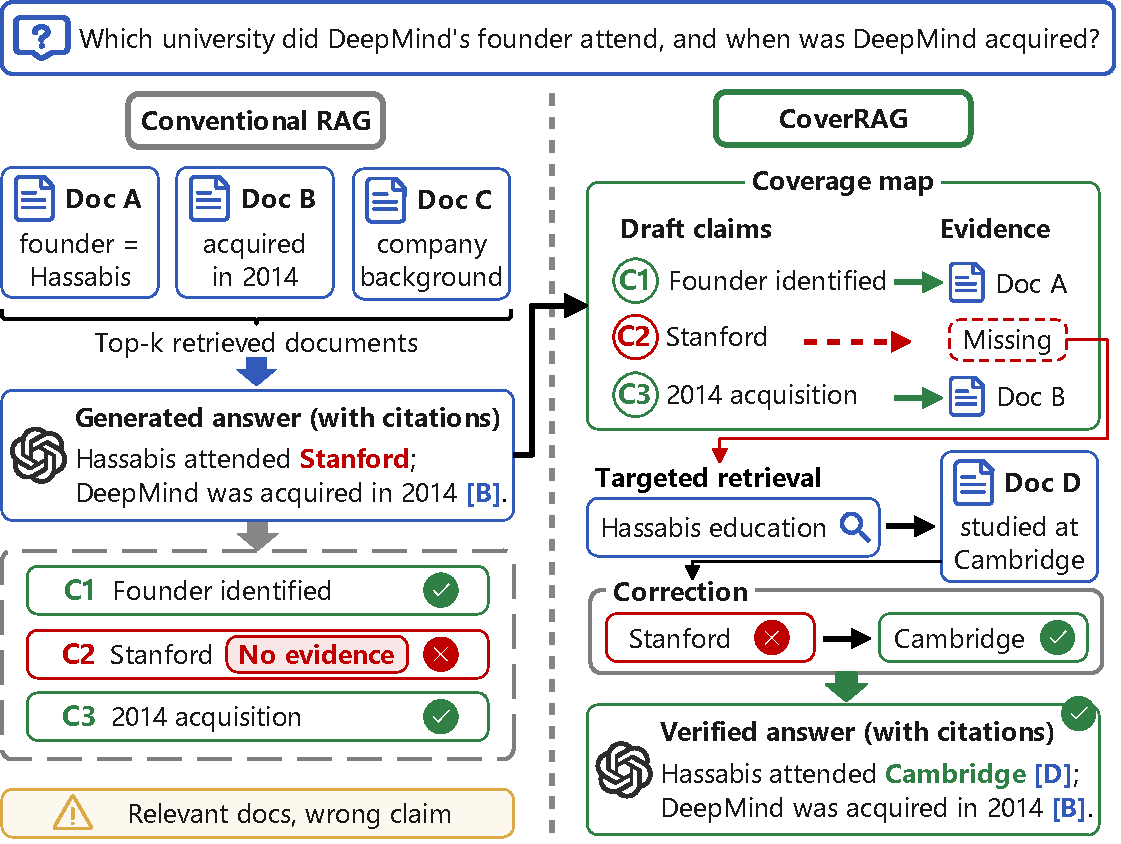
\includegraphics[width=\linewidth]{figs_wh/bg.pdf}
    \caption{Comparison of conventional RAG and \ragname.}
    % 中文图注：传统 RAG 与 \ragname 的对比。
    % 中文图注：动机示例。传统 RAG 可能检索到与问题相关的文档，但仍然生成错误且未被证据支持的事实声明。\ragname 通过 coverage map 定位该 unsupported claim，针对证据缺口发起定向检索，修正错误 claim，并生成所有关键事实声明都被引用证据覆盖的验证答案。
    \label{fig:motivation}
\end{figure}

% Existing work has addressed important parts of this problem from different angles. Strong retrievers and rerankers improve the relevance and ordering of retrieved passages~\cite{karpukhin2020dpr,izacard2021fid}. Adaptive and self-reflective RAG methods decide when to retrieve, critique intermediate generations, or correct poor retrieval results~\cite{asai2023selfrag,jeong2024adaptive_rag,yan2024crag}. Attributed generation benchmarks and citation-aware prompting evaluate whether generated answers are supported by cited sources~\cite{gao2023alce}. Knowledge-enhanced and graph-based RAG methods introduce structured data, entity relations, and graph retrieval to improve grounding over complex corpora~\cite{edge2024graphrag}. 
% However, most existing methods still operate primarily at the level of queries, documents, passages, or answer sentences. They do not explicitly formulate RAG as a control problem over the coverage relation between generated atomic claims and supporting evidence.
% % 中文：已有研究已经从不同角度解决了这一问题的若干重要部分。更强的检索器和重排序器可以提升检索段落的相关性和排序质量；自适应或自反思式 RAG 方法可以决定何时检索、批判中间生成结果，或修正低质量检索；带引用生成基准和 citation-aware prompting 可以评估生成答案是否被引用来源支持；知识增强和图增强 RAG 方法则引入结构化数据、实体关系和图检索，以提升复杂语料上的 grounding 能力。然而，大多数已有方法仍主要工作在问题、文档、段落或答案句子的层面。它们并没有将 RAG 显式建模为一个围绕“生成的原子事实声明与支持证据之间覆盖关系”的控制问题。

% This missing relation is central to trustworthy data- and knowledge-empowered GenAI. A retrieved passage can be relevant without being answer-bearing. A cited document can support one claim in a sentence while failing to support another. A multi-hop conclusion can be valid only if all required evidence links are present. Conversely, not every unsupported draft claim should trigger unbounded search: some claims should be rewritten, removed, or replaced with an abstention when evidence remains insufficient. Therefore, reliable RAG requires a mechanism that can localize evidence gaps at the claim level and decide how to spend limited retrieval and verification budget.
% % 中文：这种缺失的覆盖关系正是可信数据与知识增强生成式人工智能的关键。一个被检索到的段落可以与问题相关，但并不一定包含回答问题所需的信息；一个被引用的文档可能支持同一句子中的某个 claim，却无法支持另一个 claim；一个多跳结论只有在所有必要证据链都存在时才是有效的。反过来说，也并不是每一个未被支持的草稿 claim 都应该触发无限制搜索：有些 claim 应当被改写、删除，或者在证据仍然不足时被替换为拒答。因此，可靠的 RAG 需要一种机制，能够在 claim 层面定位证据缺口，并决定如何分配有限的检索与验证预算。

% We refer to this problem as \emph{claim-level evidence coverage}. Given a question, an external corpus, and a generated answer, the goal is to determine whether each atomic factual claim in the answer is supported by an evidence set. Support may be direct, when one evidence block entails the claim, or multi-hop, when several evidence blocks jointly entail it. Claims may also be contradicted or left with insufficient evidence. This formulation shifts the objective of RAG from merely retrieving relevant documents to covering answer-bearing claims with verifiable evidence. It also exposes a key systems challenge: verification and repeated retrieval can improve faithfulness, but they introduce additional cost and latency. The goal is not to make every answer cheaper than one-shot RAG. Instead, the goal is to allocate a bounded evidence budget to the claims that most need it, avoiding unnecessary retrieval for already supported claims and avoiding wasteful attempts to rescue low-value or unverifiable claims.
% % 中文：我们将这一问题称为 claim-level evidence coverage，即声明级证据覆盖。给定一个问题、一个外部语料库和一个生成答案，目标是判断答案中的每一个原子事实声明是否都被某个证据集合支持。这种支持可以是直接支持，即单个证据块即可蕴含该 claim；也可以是多跳支持，即多个证据块共同蕴含该 claim。某些 claim 也可能被证据反驳，或者处于证据不足状态。这一形式化将 RAG 的目标从“检索相关文档”转向“用可验证证据覆盖答案中的关键事实声明”。同时，它也暴露了一个关键系统挑战：验证和重复检索可以提升忠实性，但也会引入额外成本和延迟。因此，我们的目标并不是让每个答案都比一次性 RAG 更便宜，而是在有限证据预算下，将额外计算分配给最需要它的 claim，避免对已经被支持的 claim 进行不必要检索，也避免浪费资源去挽救低价值或不可验证的 claim。

Existing work has improved RAG from several directions, including stronger retrieval and reranking~\cite{karpukhin2020dense,izacard2021leveraging}, adaptive or self-reflective retrieval control~\cite{asai2024self,jeong2024adaptive,yan2024corrective}, and knowledge- or graph-enhanced grounding~\cite{edge2024local}. 
However, these methods mainly optimize query-level retrieval decisions, document or passage relevance, or structured context construction. They do not explicitly model whether each atomic factual claim in the final answer is covered by sufficient and verifiable evidence.
% 中文：已有工作已经从多个方向改进 RAG，包括更强的检索与重排序、自适应或自反思式检索控制、带引用生成与评估，以及知识增强或图增强的 grounding。然而，这些方法主要优化的是 query-level 的检索决策、文档或段落相关性、句子级引用质量，或结构化上下文构建。它们并没有显式建模最终答案中的每一个原子事实声明是否都被充分且可验证的证据覆盖。

We refer to this missing objective as \emph{claim-level evidence coverage}. Given a generated answer, the goal is to verify whether its atomic factual claims are supported, contradicted, or insufficiently evidenced by the retrieved corpus. This formulation shifts RAG from retrieving relevant documents to ensuring that answer-bearing claims are grounded in verifiable evidence. It also introduces a practical systems challenge: additional retrieval and verification can improve faithfulness, but must be selectively allocated under bounded cost and latency.
% 中文：我们将这一缺失目标称为 claim-level evidence coverage，即声明级证据覆盖。给定一个生成答案，系统需要验证其中的原子事实声明是否被检索语料支持、被证据反驳，或处于证据不足状态。这一形式化将 RAG 的目标从检索相关文档转向确保答案中的关键事实声明被可验证证据支撑。同时，它也带来一个实际的系统挑战：额外的检索与验证虽然可以提升忠实性，但必须在有限成本和延迟约束下有选择地分配。

% To address this problem, we propose \textsc{CoverRAG}, a \textbf{C}laim-\textbf{O}riented \textbf{V}erification and \textbf{E}vidence-\textbf{R}outed \textbf{R}etrieval-\textbf{A}ugmented \textbf{G}eneration framework. \ragname is designed as a controller layer that can be placed over different retrieval backends, including sparse retrieval, dense retrieval, hybrid retrieval, rerankers, and structured knowledge retrievers. It first diagnoses the query and decomposes it into information needs, or slots, rather than immediately committing to answer claims. It then retrieves and screens candidate evidence, generates a draft answer, decomposes the draft into atomic factual claims, and verifies each claim against the available evidence. The verification results are organized into a claim-evidence coverage map that records supported, multi-hop supported, contradicted, and insufficiently supported claims. For critical evidence gaps, \ragname performs targeted retrieval using claim-specific or slot-specific queries. Finally, it generates the answer under citation constraints, allowing only supported or multi-hop supported claims to appear in the final response and requiring unsupported critical information to be omitted or explicitly marked as insufficiently evidenced.
% % 中文：为了解决这一问题，我们提出 \ragname，即面向事实声明验证与证据路由的检索增强生成框架。\ragname 被设计为一个 controller layer，可以叠加在不同检索后端之上，包括稀疏检索、稠密检索、混合检索、重排序器以及结构化知识检索器。它首先诊断用户问题，并将问题拆解为信息需求或 slots，而不是一开始就直接生成答案 claim。随后，系统检索并筛选候选证据，生成草稿答案，将草稿拆解为原子事实声明，并针对可用证据逐条验证这些 claim。验证结果被组织成一张 claim-evidence coverage map，用来记录被支持、多跳支持、被反驳和证据不足的 claim。对于关键证据缺口，\ragname 使用 claim-specific 或 slot-specific 查询进行定向检索。最后，系统在引用约束下生成最终答案，只允许被支持或多跳支持的 claim 出现在最终回答中，并要求未被支持的关键信息被省略，或明确标注为证据不足。

% The central design principle of \ragname is that verification should not be used only as a post-hoc evaluator. Instead, verification should guide retrieval, evidence selection, answer revision, and citation control. This principle distinguishes \ragname from pipelines that retrieve a larger context window, ask the LLM to self-reflect, or evaluate citations after generation. By using the coverage map as an intermediate data structure, \ragname can localize failure modes: whether a wrong answer arises from missing evidence, irrelevant evidence, conflicting evidence, verifier uncertainty, citation mismatch, or unsupported generation. This makes the system not only more faithful, but also more auditable.
% % 中文：\ragname 的核心设计原则是：验证不应只作为生成后的评估器使用。相反，验证结果应当反过来指导检索、证据选择、答案修订和引用控制。这一点使 \ragname 区别于那些仅仅扩大上下文窗口、让 LLM 自我反思，或在生成后再评估引用的流水线。通过将 coverage map 作为中间数据结构，\ragname 可以定位不同类型的失败原因：错误答案究竟来自缺失证据、无关证据、冲突证据、验证器不确定性、引用不匹配，还是生成模型引入了未被支持的内容。因此，该系统不仅更忠实于证据，也更具可审计性。

To address this problem, we propose \textsc{CoverRAG}, a \textbf{C}laim-\textbf{O}riented \textbf{V}erification and \textbf{E}vidence-\textbf{R}outed \textbf{R}etrieval-\textbf{A}ugmented \textbf{G}eneration framework. \ragname is designed as a controller layer over heterogeneous retrieval backends. Rather than treating verification as a post-hoc evaluator, \ragname uses verification as a control signal throughout the generation process. It decomposes information needs and draft answers into verifiable units, checks whether atomic factual claims are supported by available evidence, and organizes the results into a claim-evidence coverage map. This map enables the system to localize evidence gaps, route targeted retrieval for unsupported critical claims, revise or omit insufficiently grounded content, and generate final answers under citation constraints. In this way, \ragname shifts RAG from a retrieve-then-generate pipeline toward a verification-guided process in which retrieval, evidence selection, answer revision, and citation control are jointly driven by claim-level evidence coverage.
% 中文：为了解决这一问题，我们提出 \textsc{CoverRAG}，即面向事实声明验证与证据路由的检索增强生成框架。\ragname 被设计为一个位于异构检索后端之上的 controller layer，可支持稀疏检索、稠密检索、混合检索、基于重排序的检索以及结构化知识检索。与将验证仅作为生成后评估器不同，\ragname 将验证结果作为贯穿生成过程的控制信号。它将信息需求和草稿答案分解为可验证单元，检查原子事实声明是否被已有证据支持，并将结果组织为 claim-evidence coverage map。基于该覆盖图，系统能够定位证据缺口，针对未被支持的关键 claim 发起定向检索，修订或删除证据不足的内容，并在引用约束下生成最终答案。由此，\ragname 将 RAG 从传统的“先检索、再生成”流程推进为一种 verification-guided 的过程，使检索、证据选择、答案修订和引用控制都由 claim-level evidence coverage 共同驱动。

We evaluate \ragname on long-form question answering, multi-hop question answering, and attributed generation tasks using both standard and stress-test settings. The evaluation jointly measures answer correctness, citation faithfulness, unsupported claim rate, weighted evidence coverage, token cost, retrieval calls, verifier calls, and latency. This evaluation design is important because improvements in faithfulness should not be obtained merely by generating longer answers, retrieving more documents without control, or abstaining excessively. Instead, a trustworthy RAG system should improve the alignment between answer claims and evidence while maintaining useful answers under realistic resource constraints.
% 中文：我们将在长答案问答、多跳问答和带引用生成任务上评估 \ragname，并同时采用标准设置和压力测试设置。评估指标将联合考察答案正确性、引用忠实性、未支持 claim 比例、加权证据覆盖率、token 成本、检索调用次数、验证器调用次数和延迟。这样的评估设计非常重要，因为忠实性的提升不应仅仅来自生成更长答案、无控制地检索更多文档，或过度拒答。相反，一个可信 RAG 系统应当在现实资源约束下提升答案 claim 与证据之间的对齐程度，同时保持答案的有用性。

This paper makes the following contributions:

\begin{itemize}
    \item We formulate \emph{claim-level evidence coverage} as a data- and knowledge-centric objective for trustworthy retrieval-augmented generation, bridging the gap between document-level relevance and claim-level faithfulness.
    % 中文：贡献一：将声明级证据覆盖形式化为可信检索增强生成中的一个以数据和知识为中心的目标，从而弥合文档级相关性与答案级忠实性之间的差距。
    \item We propose \textsc{CoverRAG}, a verification-guided and evidence-routed framework that decomposes answers into atomic claims, verifies each claim against evidence, builds a claim-evidence coverage map, performs targeted retrieval for evidence gaps, and generates citation-constrained final answers.
    % 中文：贡献二：提出 \ragname，一个由验证引导、由证据路由驱动的框架，它将答案拆解为原子 claim，逐条验证 claim 与证据之间的关系，构建 claim-evidence coverage map，针对证据缺口执行定向检索，并生成受引用约束的最终答案。
    \item We introduce an evaluation protocol that jointly considers answer correctness, citation faithfulness, unsupported claim rate, evidence coverage, cost, and latency, enabling a more complete assessment of reliable RAG systems.
    % 中文：贡献三：提出一个联合评估协议，同时考察答案正确性、引用忠实性、未支持 claim 比例、证据覆盖率、成本和延迟，从而更全面地评估可靠 RAG 系统。
    \item We provide empirical and qualitative analyses showing how claim-level coverage improves robustness under incomplete, noisy, and conflicting retrieval conditions, and how coverage maps support interpretable failure localization.
    % 中文：贡献四：通过定量和定性分析展示，claim-level coverage 如何在证据不完整、检索噪声和证据冲突等条件下提升鲁棒性，以及 coverage map 如何支持可解释的失败定位。
\end{itemize}

Overall, \ragname advances the view that data and knowledge empower GenAI not merely by being retrieved, but by being organized, verified, routed, and enforced at generation time. The next step for reliable RAG is therefore not only to retrieve more relevant documents, but to ensure that the final answer's factual claims are covered by verifiable evidence.
% 中文：总体而言，\ragname 强调这样一种观点：数据和知识赋能生成式人工智能，并不只是因为它们被检索出来，而是因为它们能够在生成过程中被组织、验证、路由并强制执行。因此，可靠 RAG 的下一步不只是检索更多相关文档，而是确保最终答案中的事实声明都被可验证证据覆盖。
